\subsection{Images}
\label{sec:images}

\paragraph{Image popularity}
%
Figure~\ref{fig-pop} shows the repository popularity distribution on May 31st.
The x-axies show the pull count (i.e., total number of pulls) for repositories
by May 31th with different ranges.  
Figure~\ref{fig_pull_cnt_total} shows the
cumulative repository frequency by pull count. ~95\% of the repositories are
pulled than 1000 totally. 90\% of the repositories only have a pull count less
than 333. The greatest pull count is 654,088,410, which is official
repository~\textit{nginx}.  
Figure~\ref{fig_pull_cnt_count} shows the
repository frequency by pull count. 31,200 of repositories are not at all.
34,100 repositories are pulled only~4 times and 27,600 repositories are pulled
~37 times, which are the two peaks shown in the figure.  Overall, repository
frequency decreases with the pull count.

The skewness of two curves in figure~\ref{fig-pop} suggests that Docker hub is
a good fit for caching few popular repositories or images, which can
significantly improve the \textit{pull} or \textit{push} performance.      

\begin{figure}[!t]
	\centering
	\subfigure[CDF of repositories by pull count]{\label{fig_pull_cnt_total}
		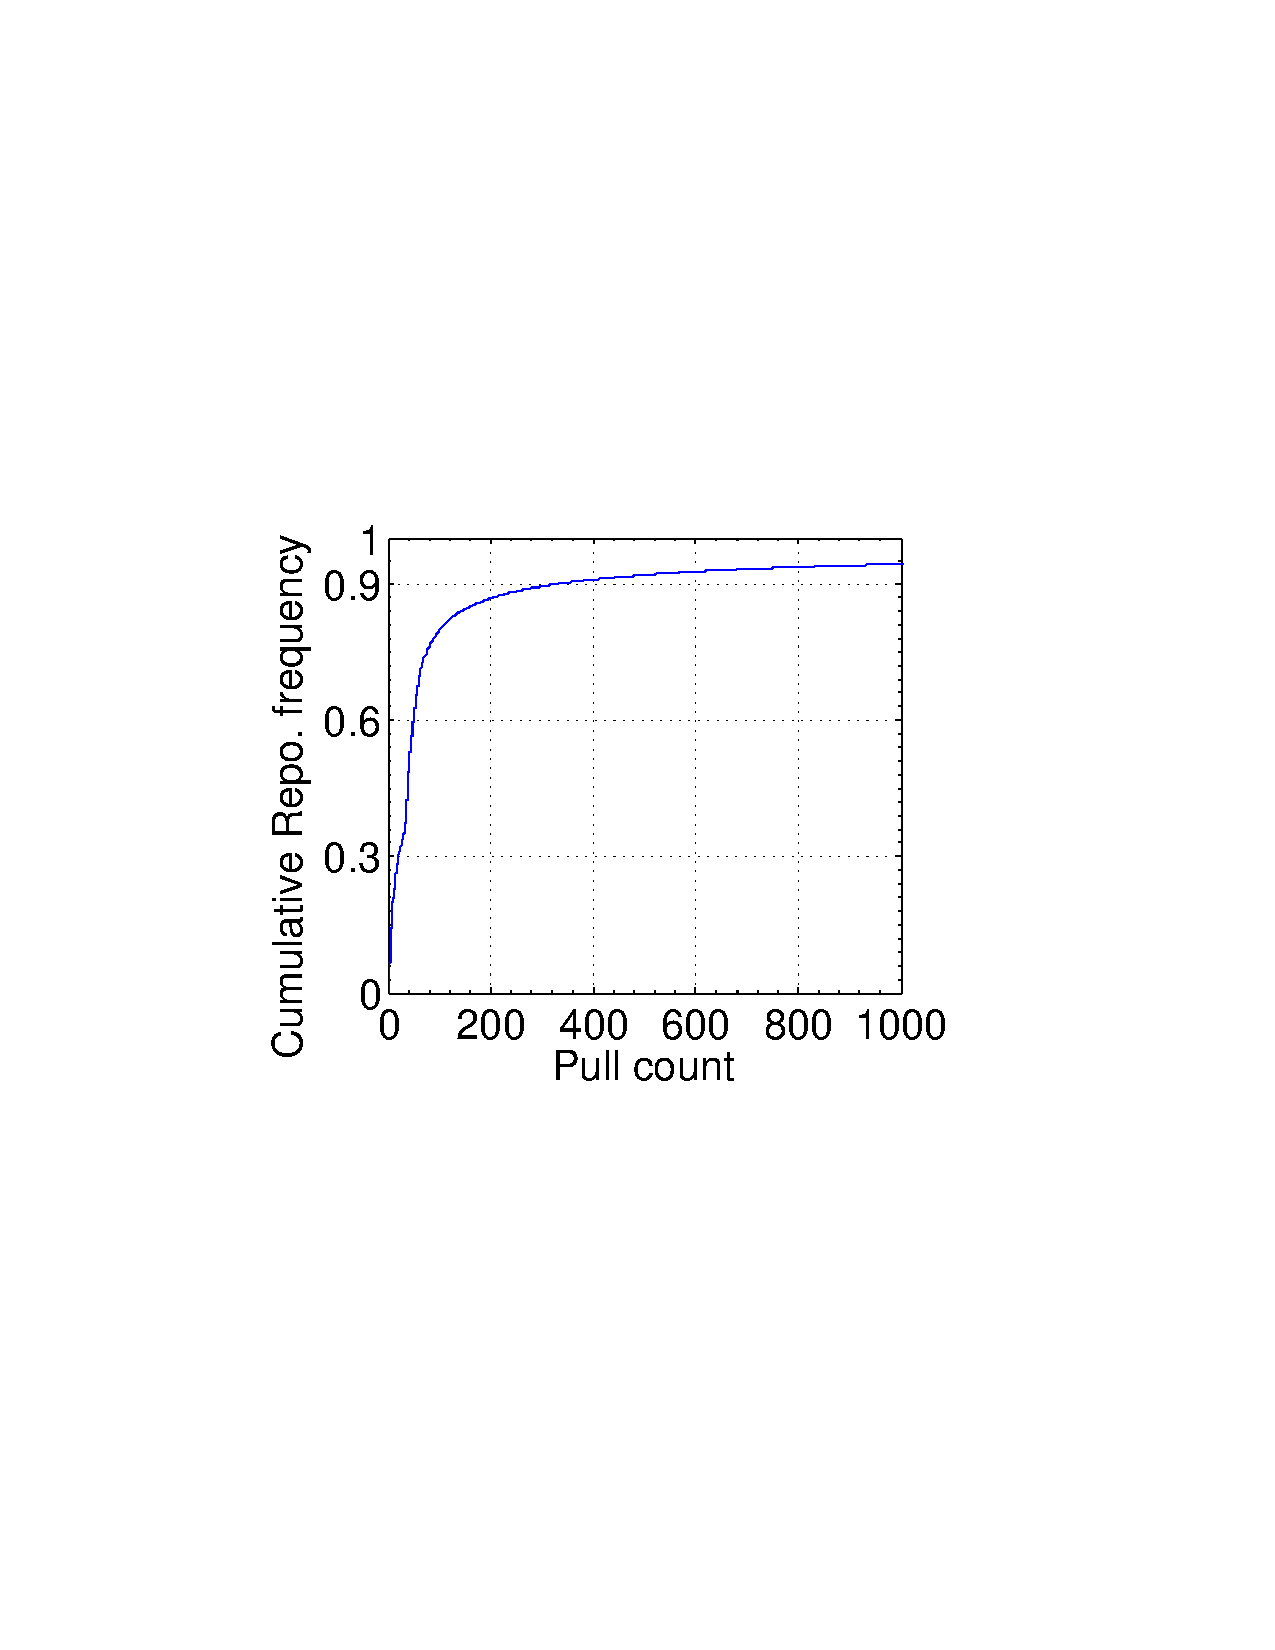
\includegraphics[width=0.23\textwidth]{graphs/pull_cnt.pdf}
	}
	\subfigure[Histogram of repositories by pull count]{\label{fig_pull_cnt_count}
		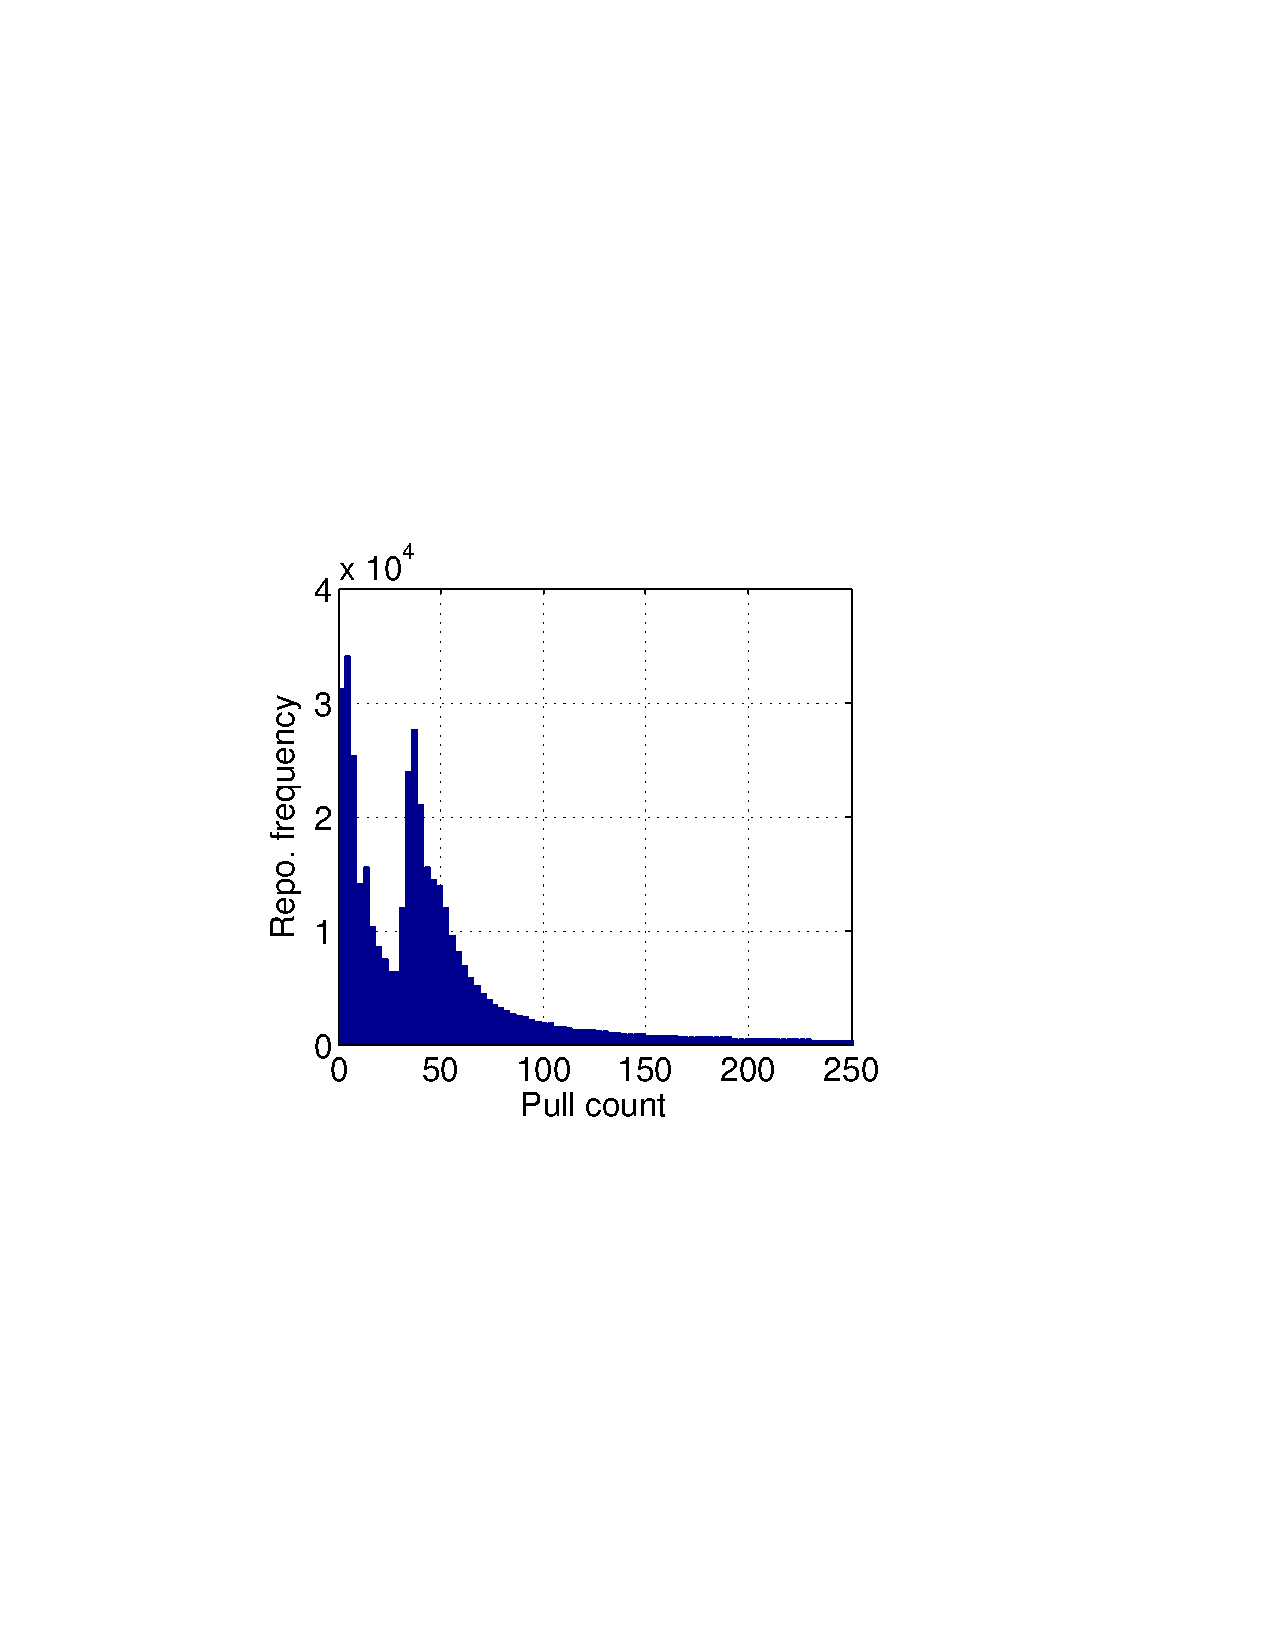
\includegraphics[width=0.22\textwidth]{graphs/count_pull_cnt.pdf}
	}
	\caption{Repository popularity distribution}
	\label{fig-pop}
\end{figure}

%%%%%%%%%%%%%%%%%%%%%%%%%%%%%%%%%%%%%%%%%%%%%%%%%%%%%%%%%%%%%%%%%%%%%
\paragraph{Image size distribution}
\label{sec:image-size}
We also measured three kinds of image size: archived image size (AIS), compressed image size (CIS), and the sum of containing file size (FIS). CIS is the sum of its containing \textit{gzip} compressed layer sizes (CLSs); AIS is the sum of its containing archived layer sizes (ALSs); FIS is the sum of its containing file sizes (FLSs).

Figure~\ref{fig-image-size} shows the cumulative image probability by three kinds of image size with different ranges.
As shown in figure~\ref{fig_image_size_gb}, The CDF distribution of images for AIS and FIS are almost similar. 90\% of images have a less than 1.3GB decompressed size for either FIS or AIS, while 90\% of images can be compressed less than 0.48 GB. The largest AIS and FIS are ~498 GB while the largest CIS is only 202 GB.
Figure~\ref{fig_image_size_mb} shows the cumulative image probability by image size in MBs. 70\% of the images can be compressed less than 190 MB. And 70\% of the images have a less than 478 MB uncompressed size (i.e., AIS or FIS). Half of the images can be compressed less than ~17 MB. Half of the images are less than 46 MB in AIS format and 94 MB in FIS formats respectively.

Figure~\ref{fig-image-size} shows that the majority of the images in Docker hub have a smaller size. 90\% of images can be compressed less than 500 MB and 70\% of images are less than 500 MB even without compression. 


\begin{figure}[!t]
	\centering
	\subfigure[CDF of images by size (GB)]{\label{fig_image_size_gb}
		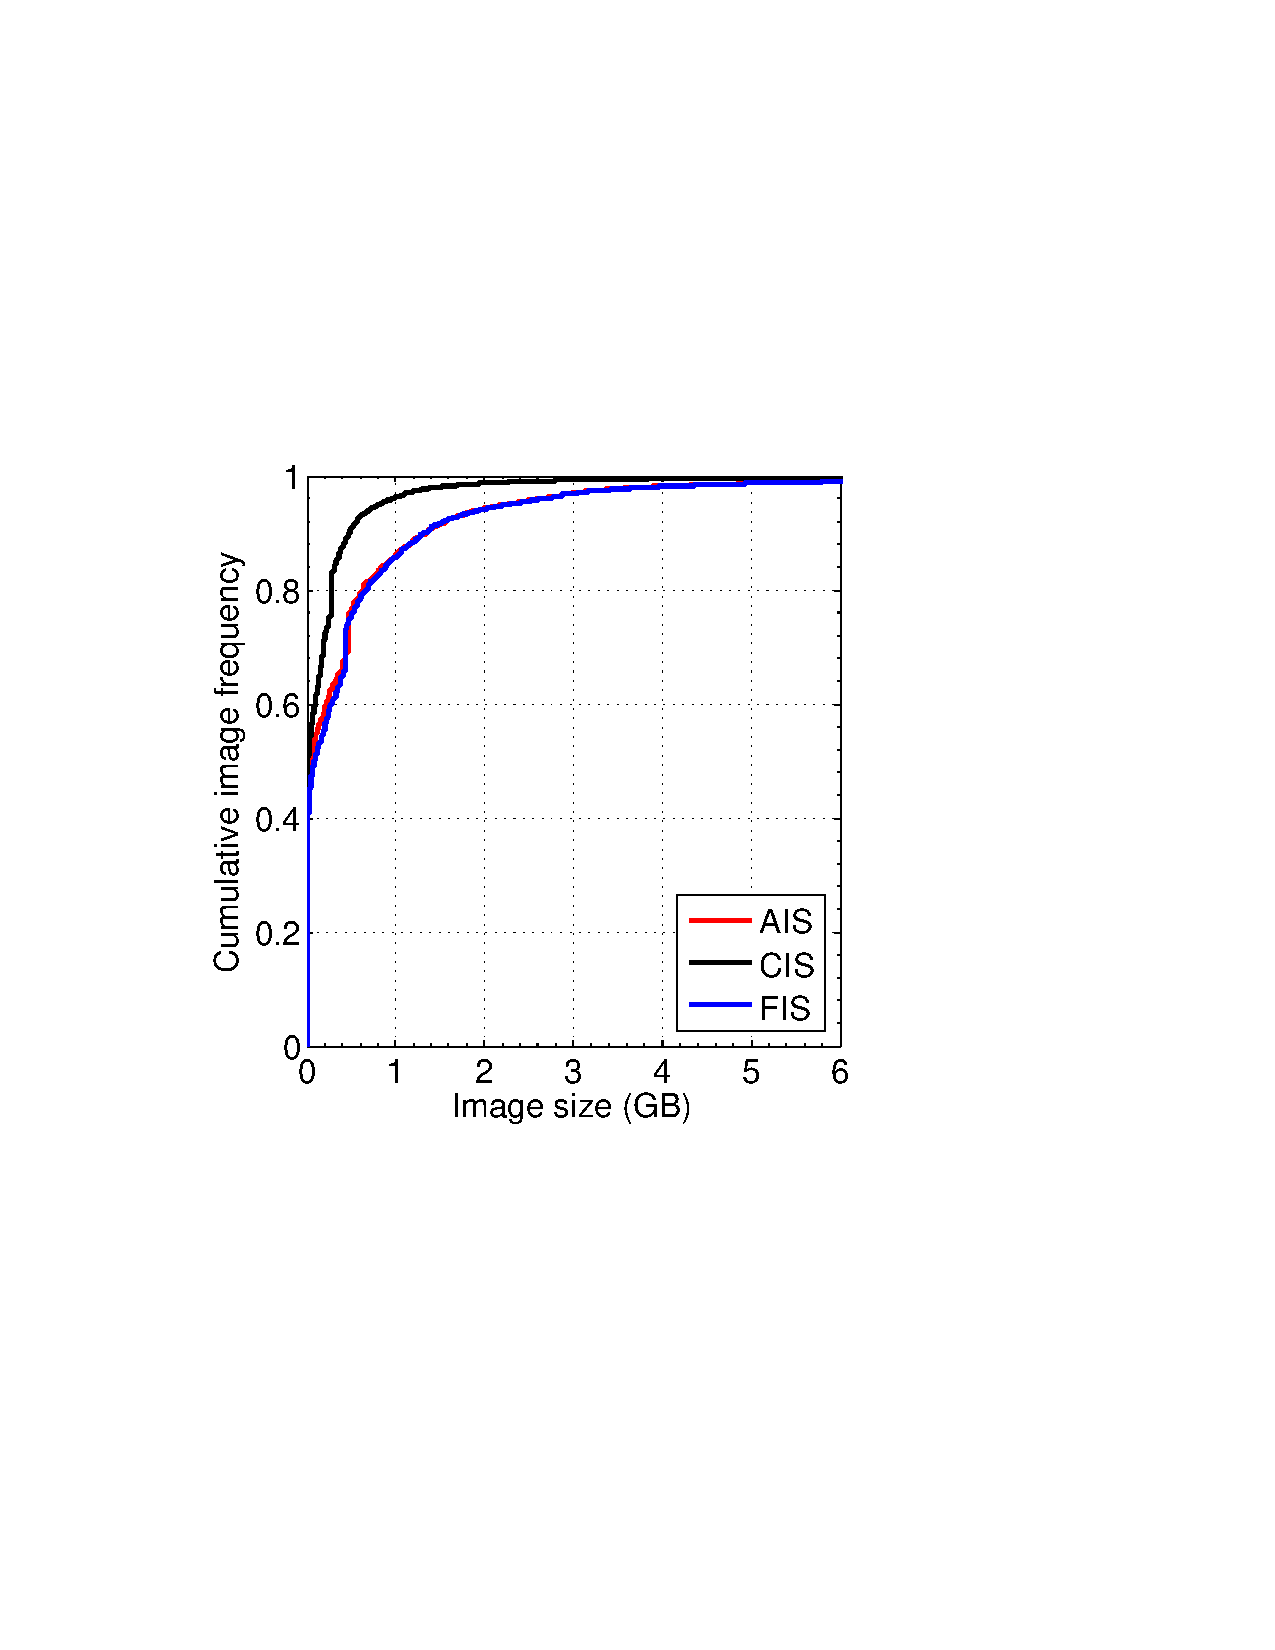
\includegraphics[width=0.22\textwidth]{graphs/size.pdf}
	}
	\subfigure[CDF of images by size (MB)]{\label{fig_image_size_mb}
		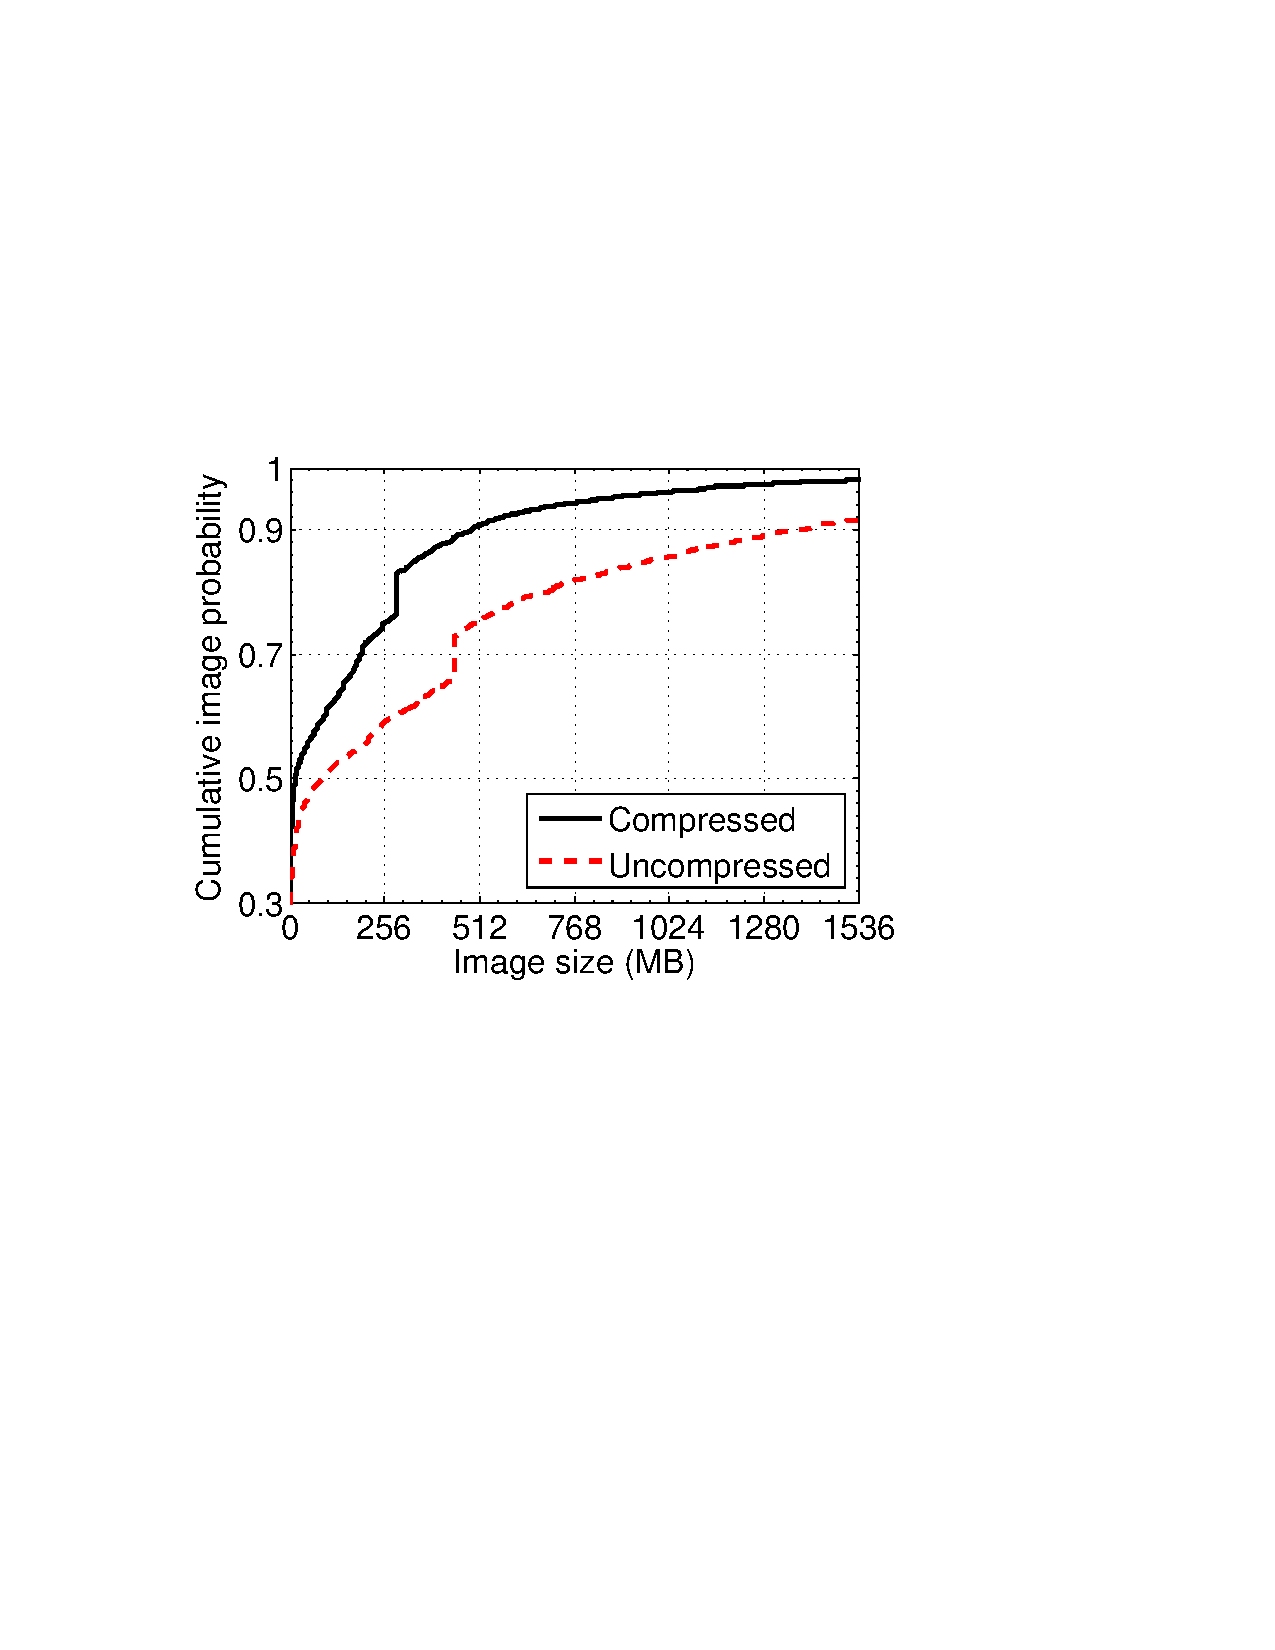
\includegraphics[width=0.23\textwidth]{graphs/size_mb.pdf}
	}
	\caption{Image size distribution}
	\label{fig-image-size}
\end{figure}

%%%%%%%%%%%%%%%%%%%%%%%%%%%%%%%%%%%%%%%%%%%%%%%%%%%%%%%%%%%%%%%%%%%%%
\paragraph{Compression rate distribution}

\begin{figure}[!t]
	\centering
	\subfigure[CDF of images by compression ratio]{\label{fig_image_compression_ratio}
		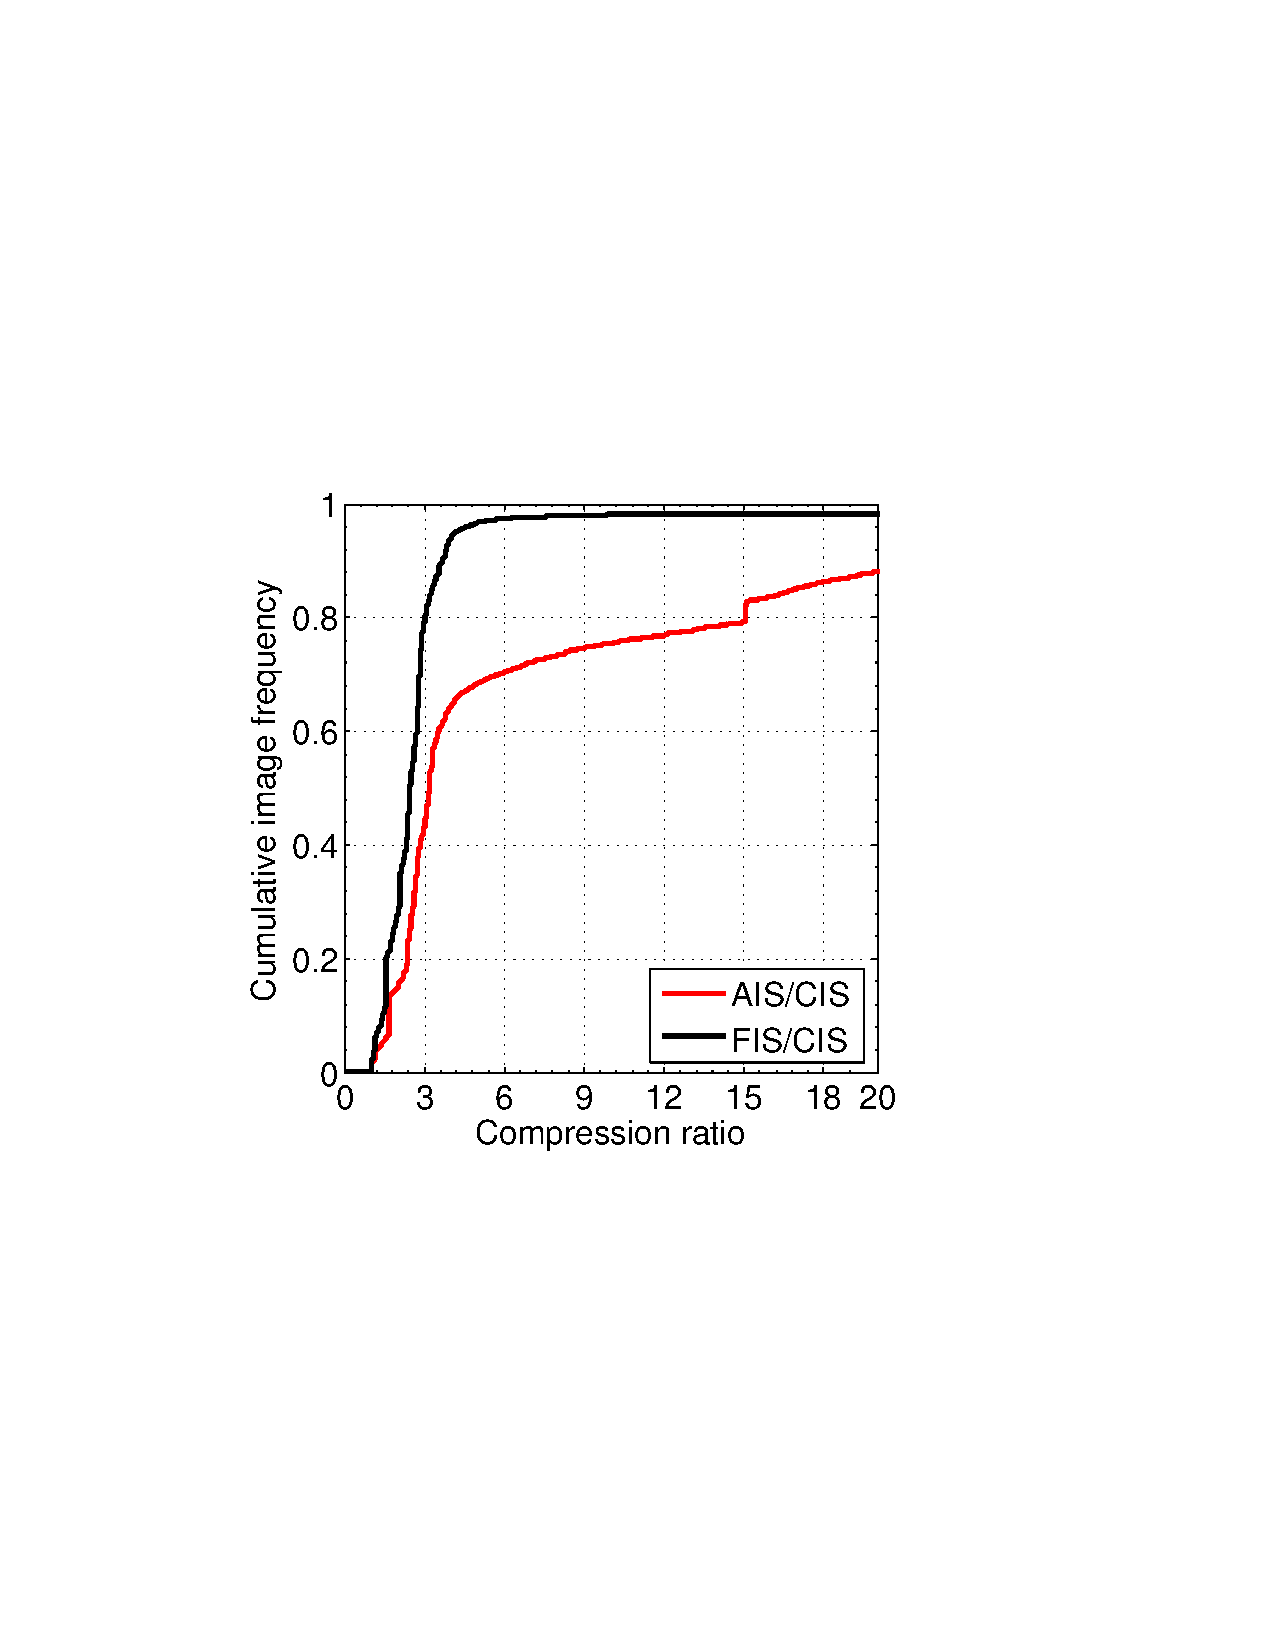
\includegraphics[width=0.23\textwidth]{graphs/compression_ratio_less.pdf}
	}
	\subfigure[Histogram of images by compression ratio]{\label{fig_image_compression_ratio_less}
		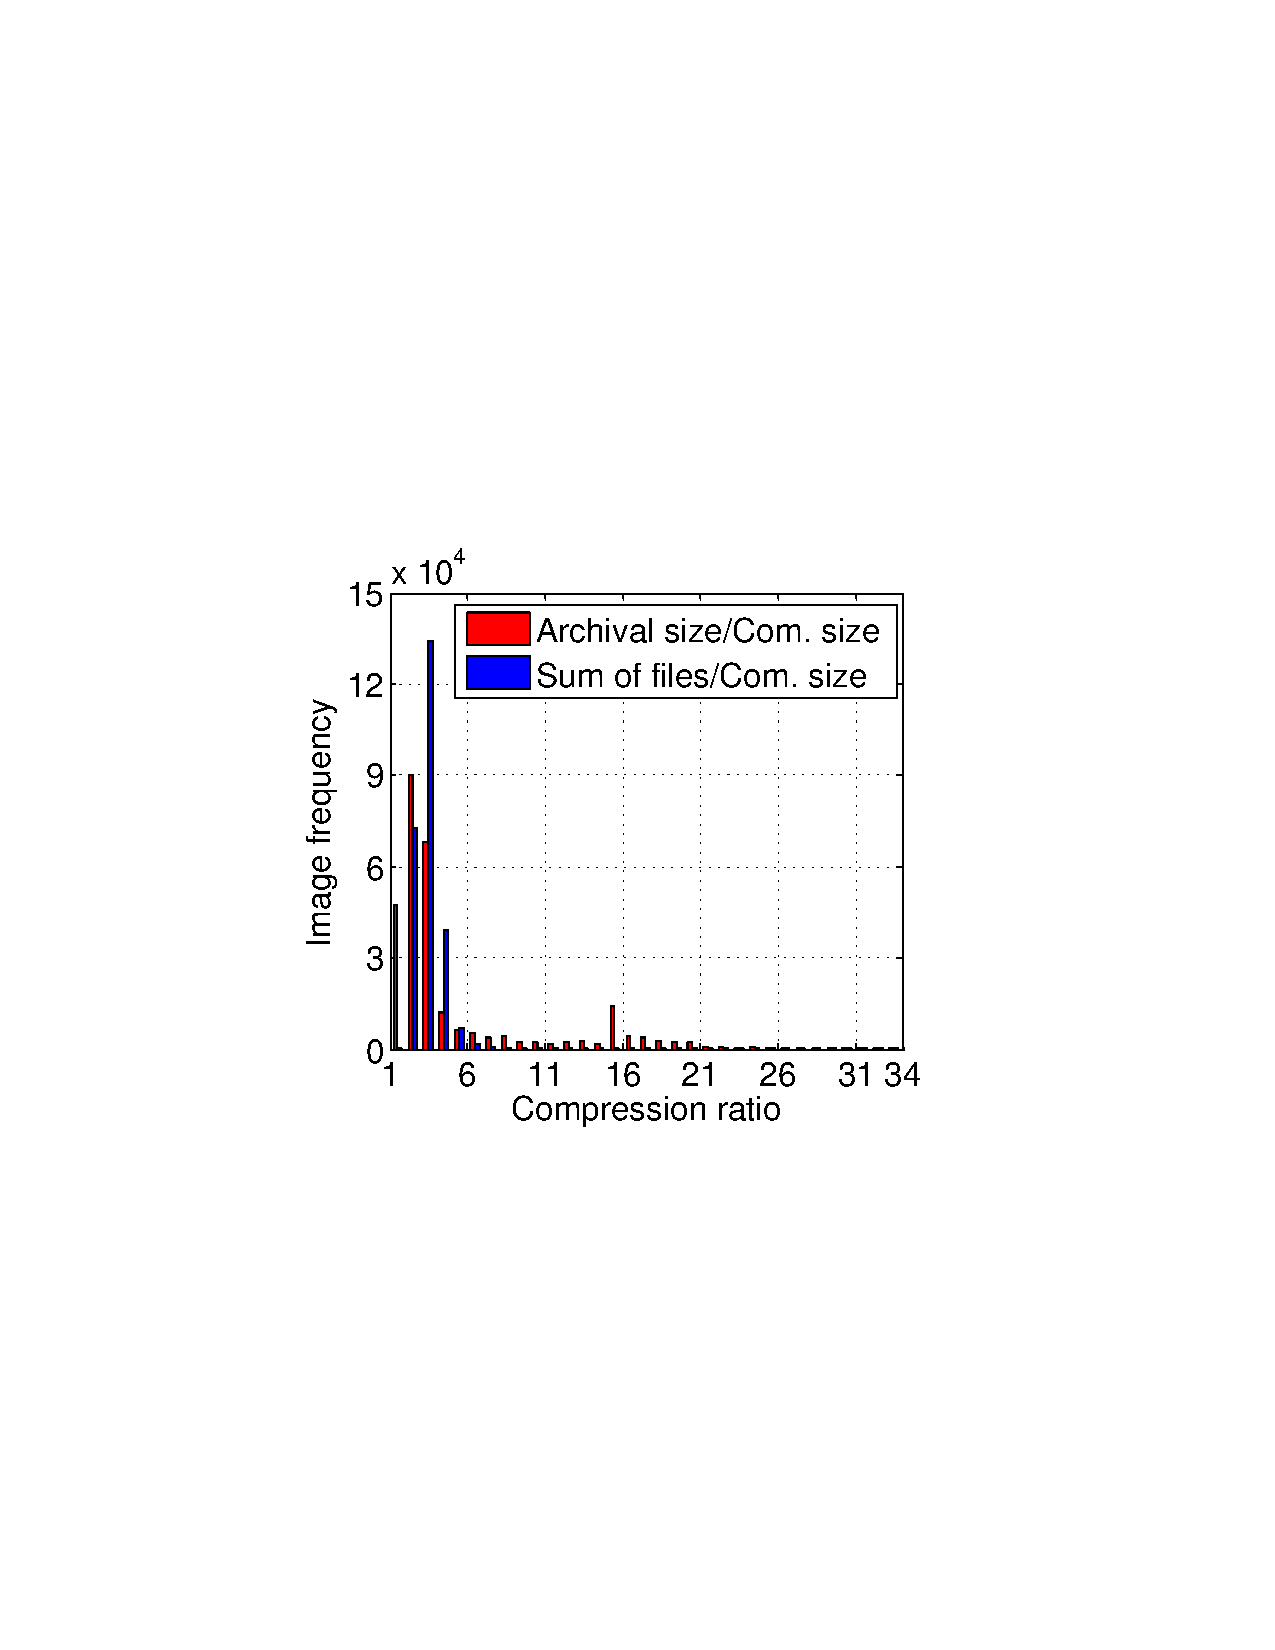
\includegraphics[width=0.223\textwidth]{graphs/hist_compression_ratio.pdf}
	}
	\caption{Compression rate distribution}
	\label{fig-image-compression-ratio}
\end{figure}

As discussed in~\ref{sec:image-size}, three kinds of image size are measured: AIS, CIS, and FIS. Thus, we calculated two kinds of compression ratio: the ratio of AIS to CIS (AIS-to-CIS) and the ratio of FIS to CIS (FIS-to-CIS). 

Figure~\ref{fig-image-compression-ratio} shows the cumulative image probability by compression ratio. Overall, we can see that AIS-to-CIS is greater than FIS-to-CIS. 90\% of images have a AIS-to-CIS less than ~4 while 90\% of images have a FIS-to-CIS less than 35. Half of the images have a compression ratio (both AIS-to-CIS and FIS-to-CIS) around 3. The maximum compression ratio are 512,930 and 1028 in FIS-CIS and AIS-CIS formats respectively.
Figure~\ref{fig_image_compression_ratio_less} shows a histogram of image probability by compression ratio. 134,000 images' FIS-to-CISs are 3.5 and 90,000 images'AIS-to-CISs are 2.5, which are two peaks shown in the graph.

Figure~\ref{fig-image-compression-ratio} suggests that Docker images has a great potential for compression to save space.
%%%%%%%%%%%%%%%%%%%%%%%%%%%%%%%%%%%%%%%%%%%%%%%%%%%%%%%%%%%%%%%%%%%%%
\paragraph{Layer count distribution}


\begin{figure}[!t]
	\centering
	\subfigure[CDF of layer count in images]{\label{fig_layer_cnt_less}
		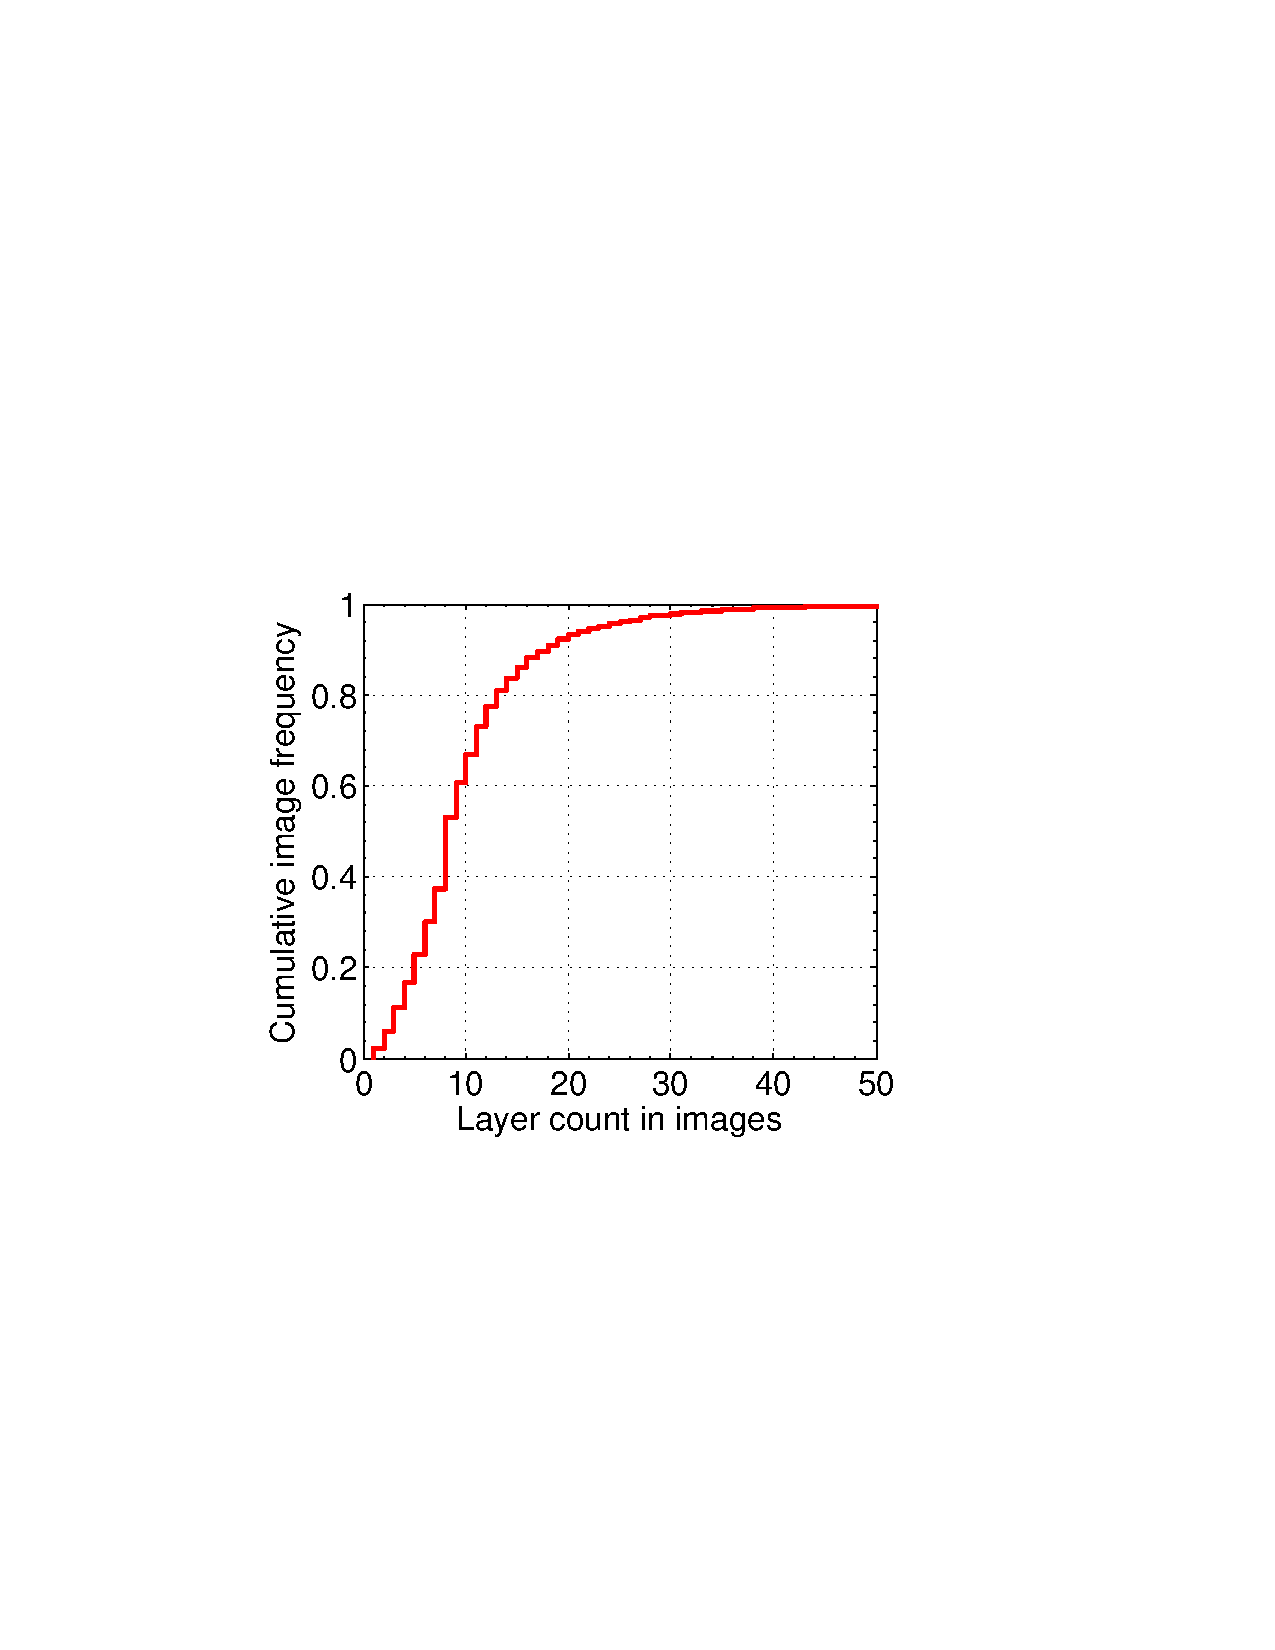
\includegraphics[width=0.23\textwidth]{graphs/layer_cnt_less.pdf}
	}
	\subfigure[Histogram of layer count in images]{\label{fig_hist_layer_cnt}
		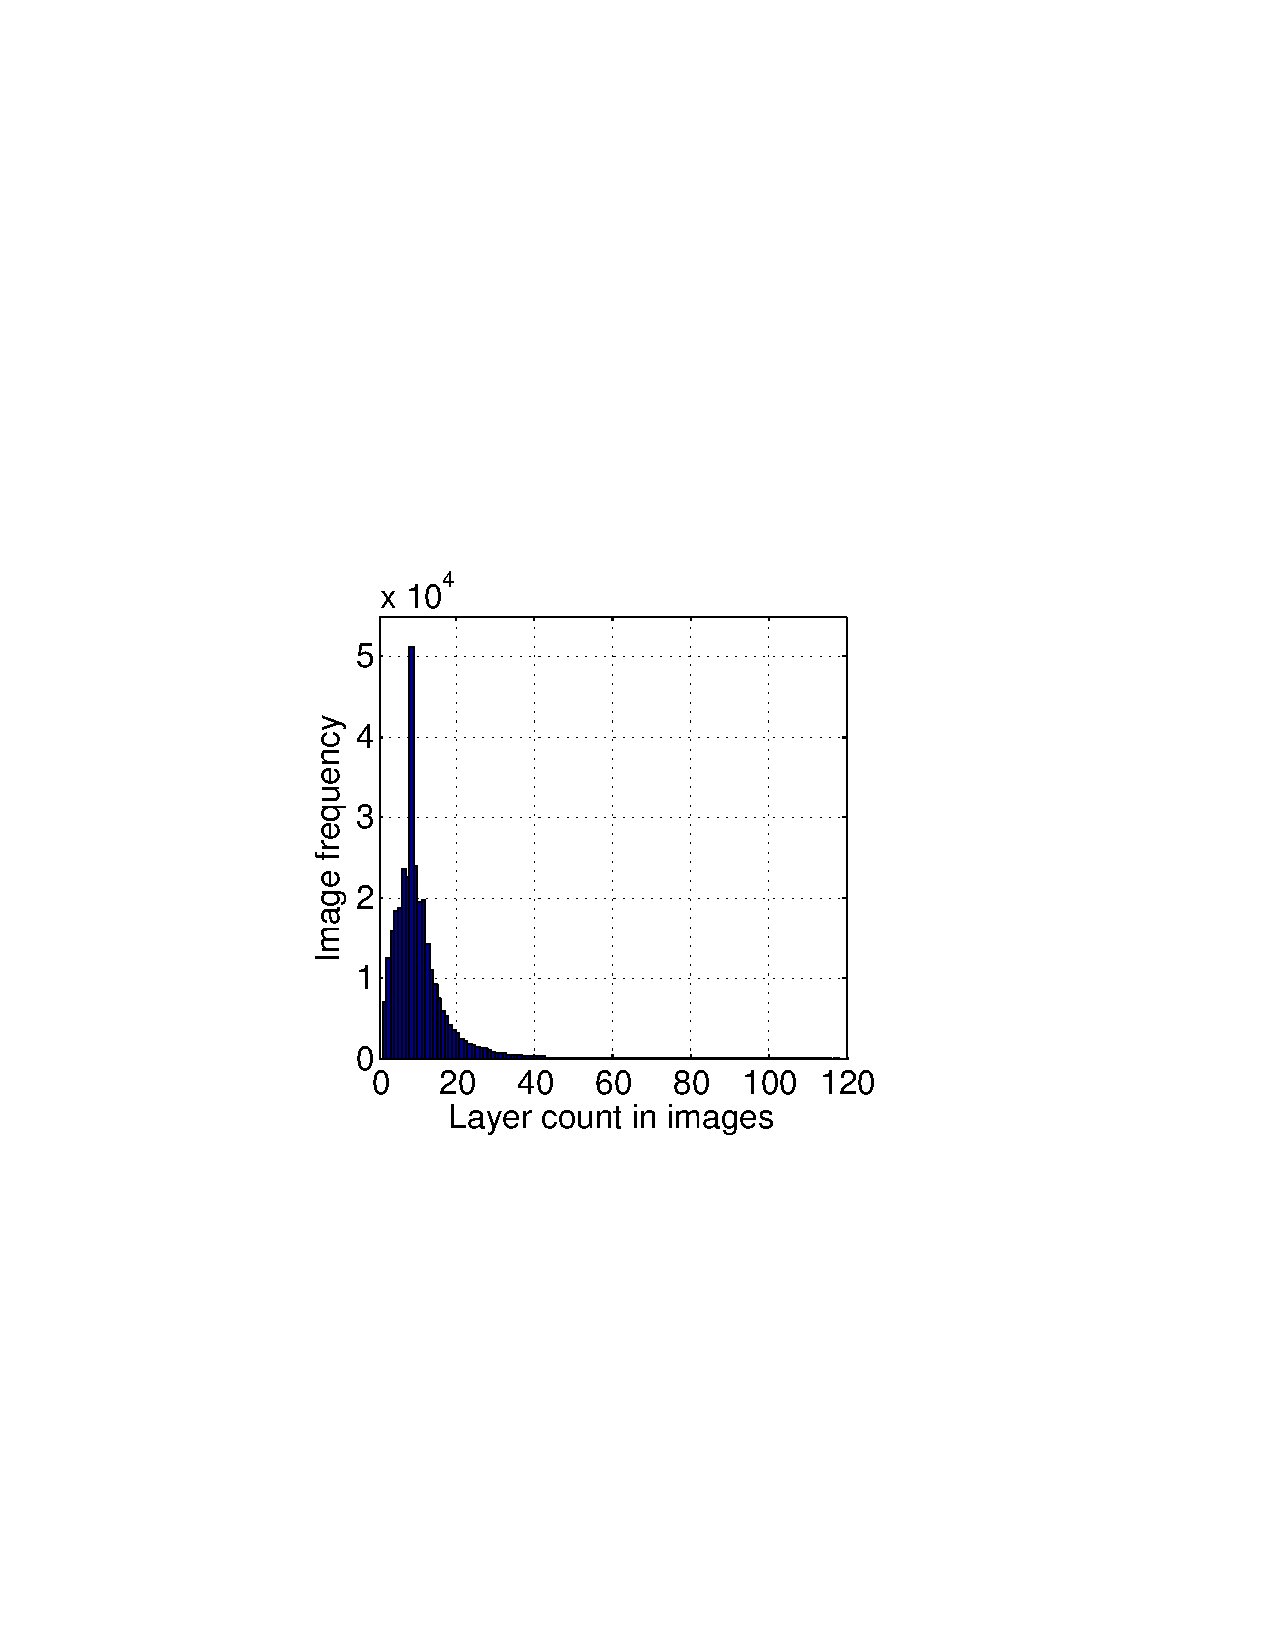
\includegraphics[width=0.213\textwidth]{graphs/hist_layer_cnt.pdf}
	}
	\caption{Layer count}
	\label{fig-layer-cnt}
\end{figure}

As discussed in~\ref{sec-image-layers}, images are consisted of a set of layers. Figure~\ref{fig-layer-cnt} shows the cumulative image probability by layer count in images. 90\% of images have less than 18 layers. Half of images have less than 8 layers. 

Figure~\ref{fig_hist_layer_cnt} shows the histogram of images by layer count in images. About 51,300 images have 8 layers, which is the peak value in the figure. The maximum layer count is 121. The average is 10. 7,060 images have only 1 layer. 

\begin{figure}[!t]
	\centering
	\subfigure[CDF of layer reference count]{\label{fig_repeate_layer}
		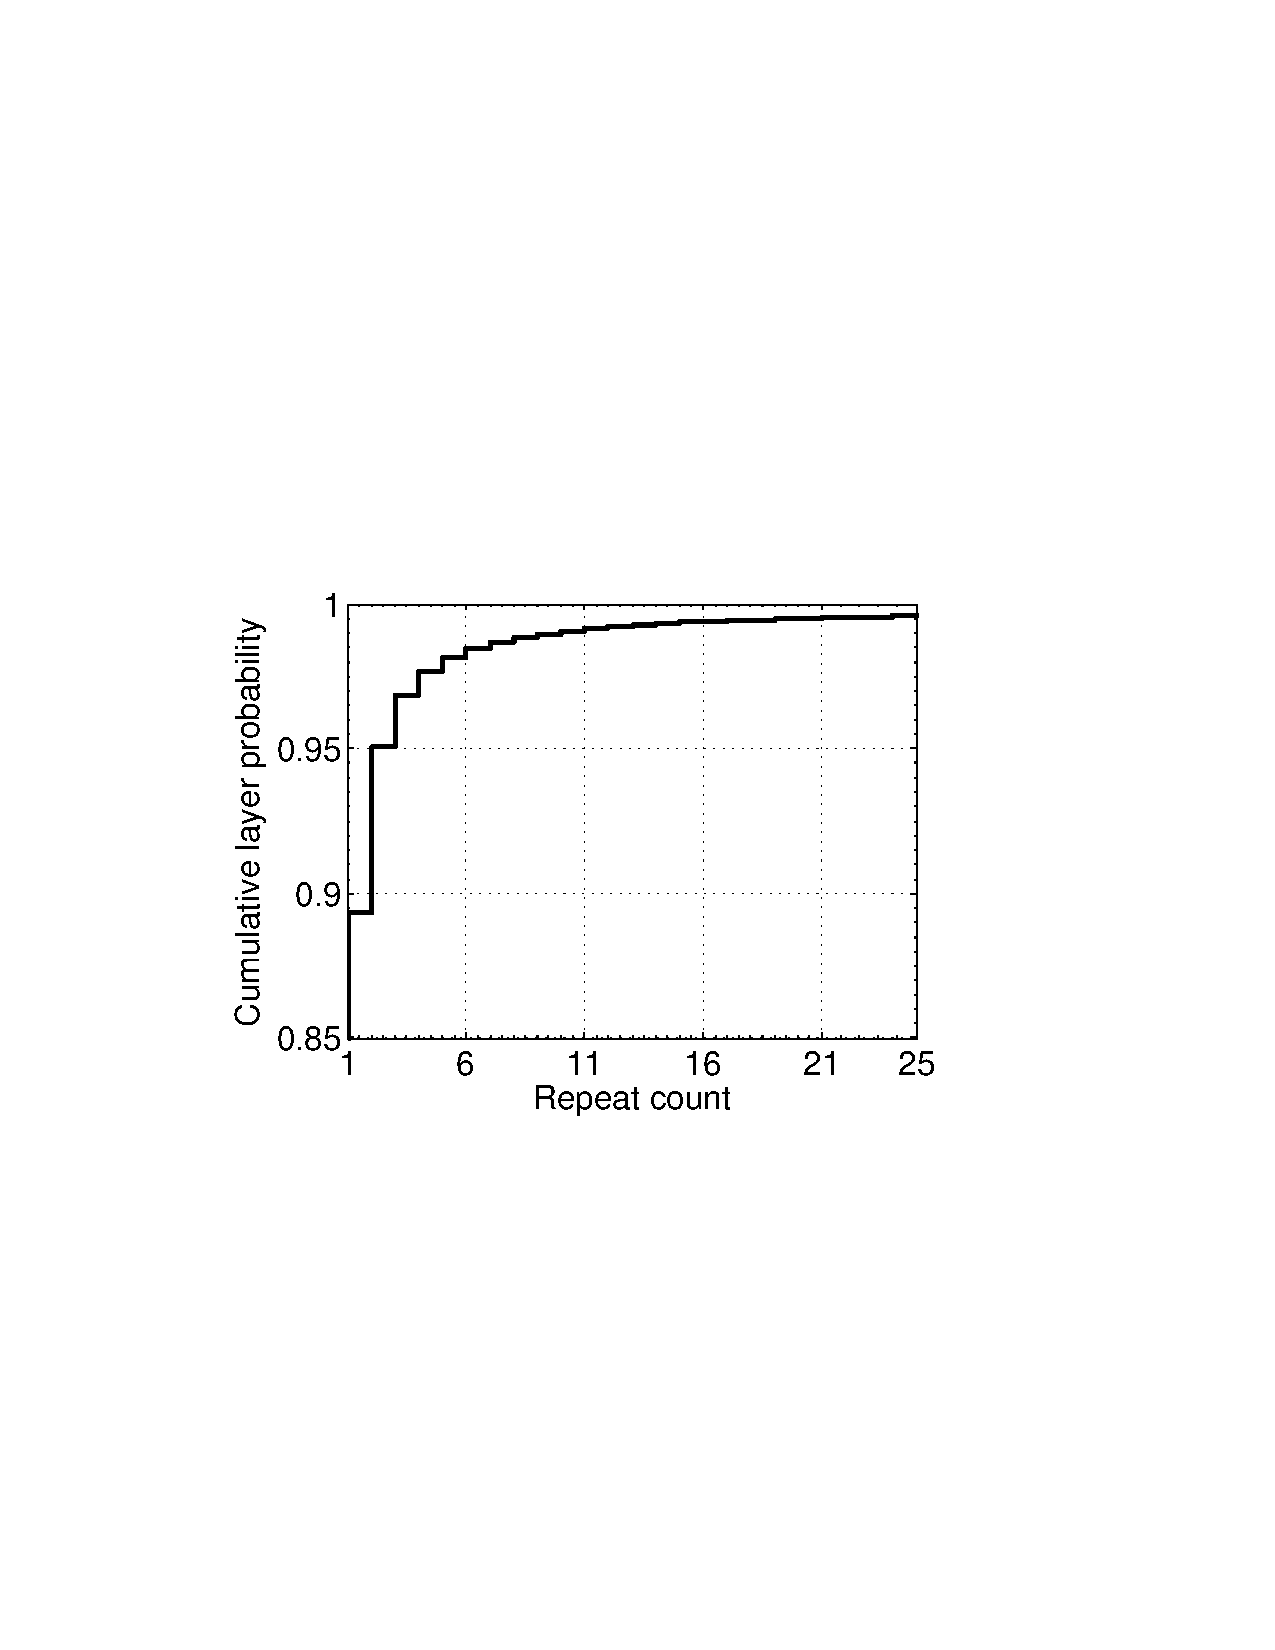
\includegraphics[width=0.23\textwidth]{graphs/repeate_layer.pdf}
	}
	\subfigure[Histogram of layer reference count]{\label{fig_hist_repeate_layer}
		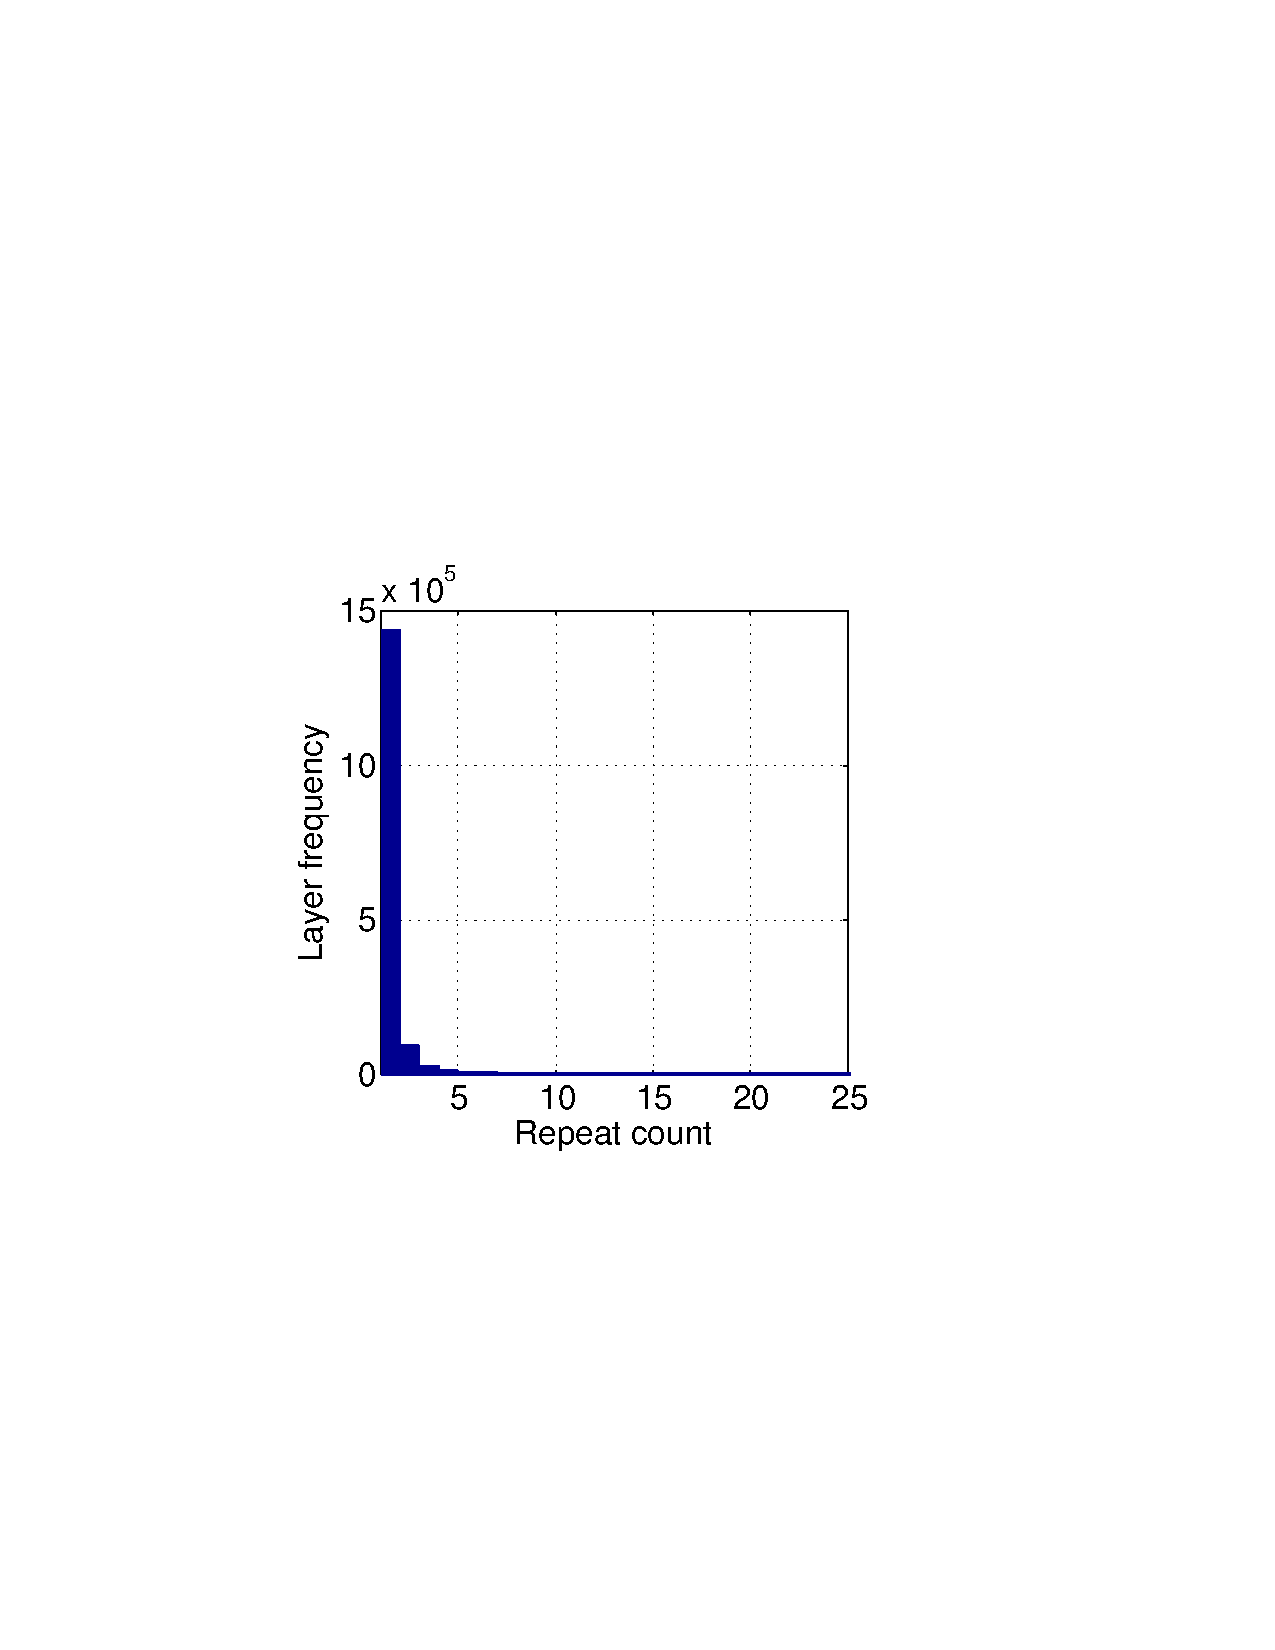
\includegraphics[width=0.223\textwidth]{graphs/hist_repeate_layer.pdf}
	}
	\caption{Layer reference counts across all images}
	\label{fig-repeat-layer-cnt}
\end{figure}
%%%%%%%%%%%%%%%%%%%%%%%%%%%%%%%%%%%%%%%%%%%%%%%%%%%%%%%%%%%%%%%%%%%%%
\paragraph{Repeat layer count distribution}

As discussed in~\ref{sec-image-layers}, layers are shared among images. Figure~\ref{fig_repeate_layer} shows the cumulative layer frequency by repeat count among images. Around 90\% of layers are only reference by a single image. 99\% of layers are shared among less than 25 images. 

Figure~\ref{fig_hist_repeate_layer} shows the histogram of layers by repeat layer count among images. About 1,440,000 layers are referenced by only one single image, which is the peak value in the figure. The maximum repeat count is 33,428 while the median is 1. The average is 2.
%%%%%%%%%%%%%%%%%%%%%%%%%%%%%%%%%%%%%%%%%%%%%%%%%%%%%%%%%%%%%%%%%%%%%
\paragraph{Directory and file count distribution}

\begin{figure}
	\centering
	\begin{minipage}{0.27\textwidth}
		\centering
		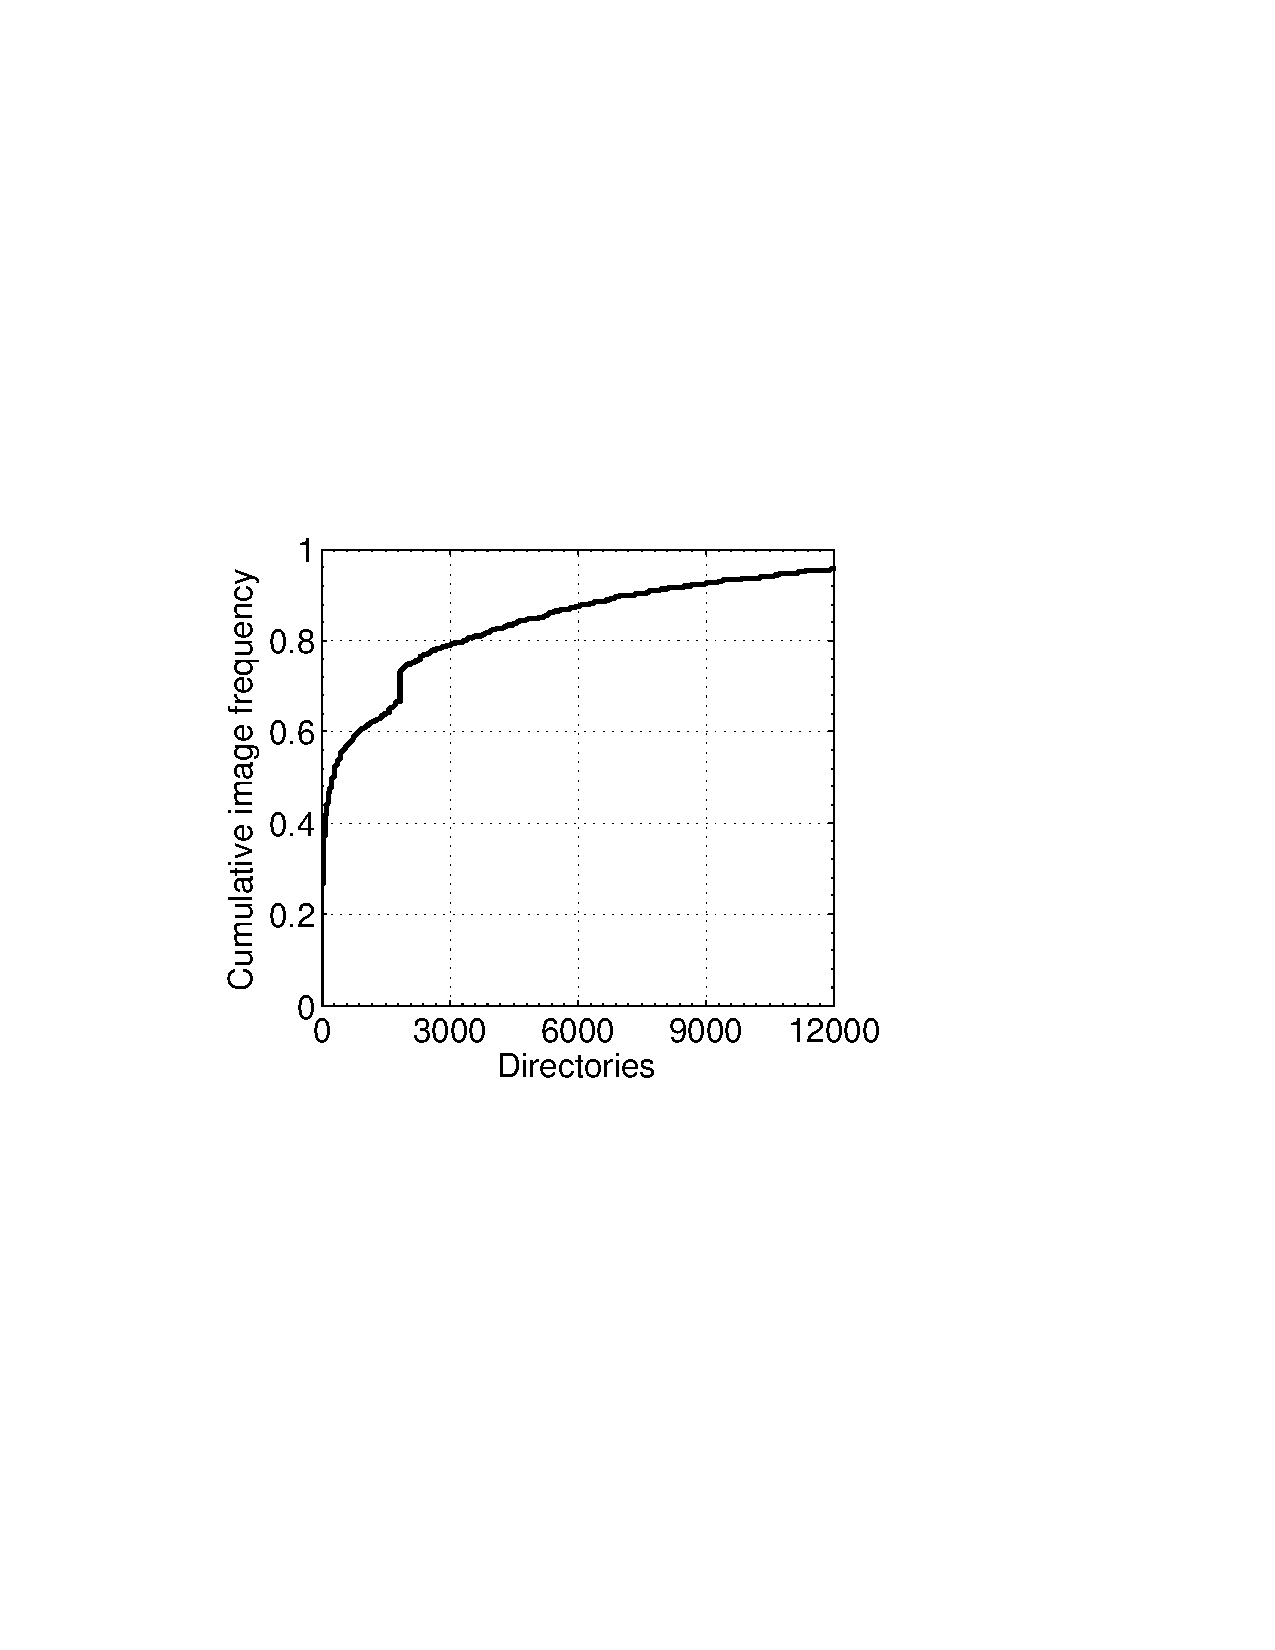
\includegraphics[width=1\textwidth]{graphs/dir.pdf}
		\caption{CDF of images by directories}
		\label{fig-dir}
	\end{minipage}%
	\begin{minipage}{0.23\textwidth}
		\centering
		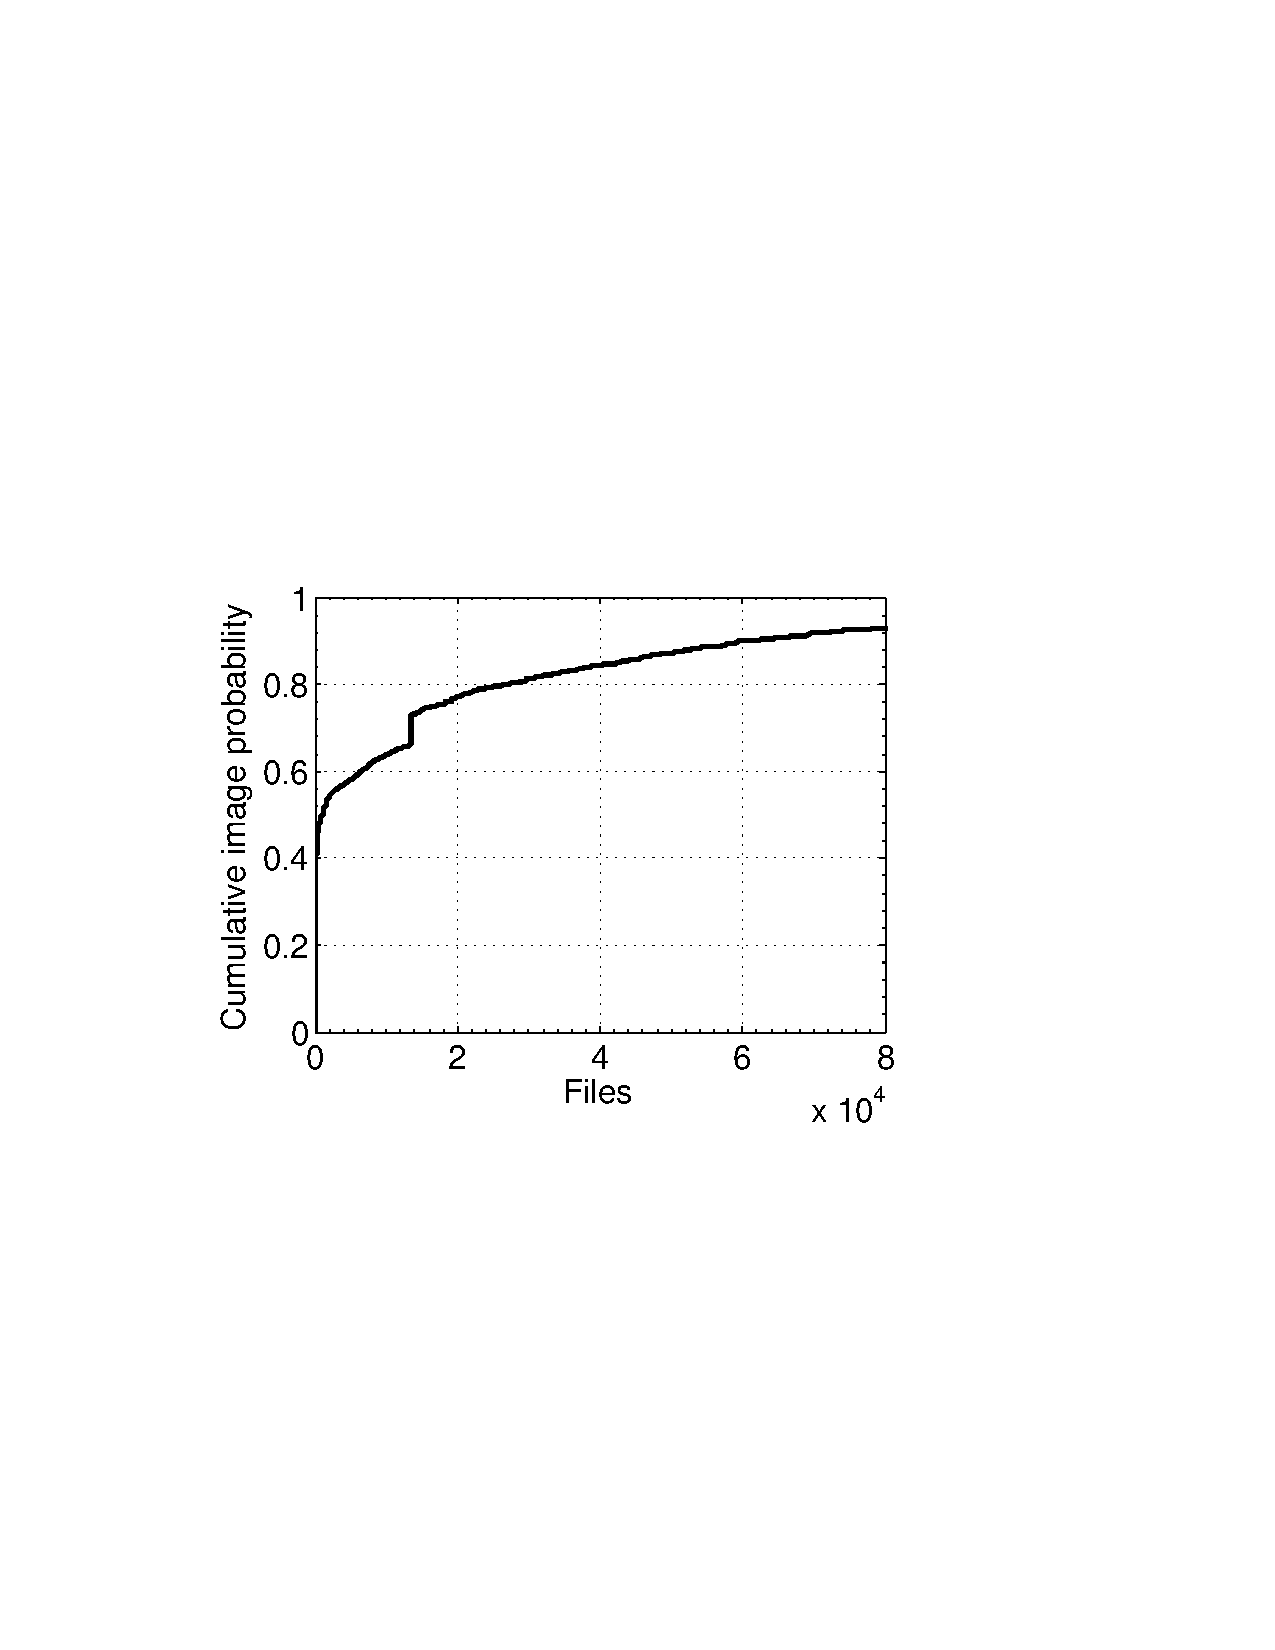
\includegraphics[width=1\textwidth]{graphs/file.pdf}
		\caption{CDF of images by files}
		\label{fig-file}
	\end{minipage}
\end{figure}

Figure~\ref{fig-dir} shows the cumulative image probability by directories. 90\% of images have less than 7,344 directories. Half of images have less than 296 directories. The maximum is 1,168,160 while the minimum is 1. The average is 2,705. 

Figure~\ref{fig-file} shows the cumulative image frequency by files. 90\% of images have less than 64,780 files. Half of images have less than 1,090 files. The maximum is 8,509,958 while the minimum is 1. The average is 21,413.
